\section{Montagem Mecânica e Elétrica da Bancada de Aquisição}

A arquitetura da bancada de aquisição foi organizada em uma estrutura funcional hierárquica, conforme apresentado no diagrama da Figura~\ref{fig:diagrama_blocos}. O sistema integra cinco camadas complementares: alimentação, controle de carga, condicionamento e medição, sensoriamento distribuído e comunicação em rede.

A energia provém de duas fontes intercambiáveis: uma bateria LiPo para operação em ensaios dinâmicos e uma fonte CA/CC de rede elétrica para operação em bancada estacionária. Ambas alimentam um barramento comum de 12V através de diodos em configuração OR lógica, garantindo que a bateria tenha prioridade automática quando conectada, sem necessidade de comutação manual. Deste barramento, dois estágios reguladores buck reduzem a tensão para 12V (alimentação de placas de controle e relés) e 5V (circuitos analógicos e sensores digitais).

O controle da conexão ao motor é realizado por dois relés em sequência: o relé de pré-carga é acionado inicialmente, inserindo um resistor de 100$\,\Omega$ em série com o barramento de alimentação do ESC, limitando a corrente de inrush durante o carregamento dos capacitores internos. Após este período de estabilização, o relé de carga é acionado, efetuando um bypass do resistor de pré-carga e conectando o ESC diretamente ao barramento de potência. Durante esta sequência, um amperímetro registra a corrente total do sistema e um voltímetro monitora continuamente a tensão da bateria.

O ESC comanda o motor BLDC, gerando três fases de corrente ($i_a$, $i_b$, $i_c$). A placa SAME captura os sinais analógicos de corrente, bem como sinais de tensão de linha para posterior reconstrução da componente de tensão neutra via transformação de Clarke.

Simultaneamente, a placa SIBA controle o PPM para acionamento do ESC, os relés de pré-carga e de carga, além das leituras, do RPM, Bateria e Tubo de pitot, via I2C (\textit{Inter-Integrated Circuit}), como também das células de carga, via \textit{bit banging} e das temperaturas da bateria e motor.

 Um switch Ethernet interno interconecta as placas SAME, SIBA e um computador externo, viabilizando aquisição sincronizada em tempo real via protocolo NCI transportado por UDP, que permite a transmissão de dados de forma isolada e com multiplos nós de operação.

\begin{figure}[htb]
    \centering
    % \includegraphics[width=0.85\textwidth]{figuras/diagrama_blocos}
    \caption{Diagrama de blocos da arquitetura de aquisição}
    \label{fig:diagrama_blocos}

    \begin{tikzpicture}[transform shape, american voltages, scale=0.7]
	% Paths, nodes and wires:
	\node[fourport, xscale=1.55, yscale=1.55](ESC) at (14.04, 9.079){} node[anchor=center] at (ESC.center){$\text{ESC}$};
	\node[fourport](N1) at (17.489, 9.039){} node[anchor=center] at (N1.center){$\text{Aquisição}$};
	\node[shape=circle, draw, line width=1pt, minimum width=1.465cm](N2) at (20.27, 9.07){} node[anchor=center] at (N2.text){$\text{BLDC}$};
	\draw (2.121, 9.949) to[battery, l={$V_{bateria}$}] (2.121, 7.449);
	\node[ground] at (2.121, 7.449){};
	\draw (2.121, 7.699) -| (2.121, 7.449);
	\draw (16.579, 9.494) |- (15.489, 9.539);
	\draw (16.579, 8.584) |- (15.489, 8.539);
	\draw (15.489, 9.039) -| (16.591, 9.017);
	\node[shape=rectangle, minimum width=0.715cm, minimum height=0.215cm](N3) at (16.114, 9.789){} node[anchor=center] at (N3.text){$i_a$};
	\node[shape=rectangle, minimum width=0.715cm, minimum height=0.215cm](N4) at (16.114, 9.289){} node[anchor=center] at (N4.text){$i_b$};
	\node[shape=rectangle, minimum width=0.715cm, minimum height=0.215cm](N5) at (16.114, 8.789){} node[anchor=center] at (N5.text){$i_c$};
	\draw (19.621, 9.449) |- (18.399, 9.494);
	\draw (19.739, 8.539) |- (18.399, 8.494);
	\draw (18.399, 8.994) -| (19.489, 9.039);
	\node[shape=rectangle, minimum width=0.715cm, minimum height=0.215cm](N6) at (19.024, 9.744){} node[anchor=center] at (N6.text){$i_a$};
	\node[shape=rectangle, minimum width=0.805cm, minimum height=0.295cm](N7) at (19.069, 9.204){} node[anchor=center] at (N7.text){$i_b$};
	\node[shape=rectangle, minimum width=0.715cm, minimum height=0.215cm](N8) at (19.024, 8.744){} node[anchor=center] at (N8.text){$i_c$};
	\draw (10.951, 10.374) to[ammeter] (11.951, 10.374);
	\draw (4.121, 8.199) to[voltmeter] (4.121, 9.449);
	\draw (7.607, 9.874) to[cute open switch, mirror, l={$\text{Relé de carga}$}] (6.107, 9.874);
	\draw (7.607, 10.874) to[cute open switch, mirror, l={$\text{Relé de pré-carga}$}] (6.107, 10.874);
	\draw (8.201, 10.874) to[american resistor, l={$100 \Omega$}] (9.951, 10.874);
	\draw (6.107, 9.874) |- (5.451, 9.874) |- (6.107, 10.874);
	\draw (7.607, 10.874) -- (8.201, 10.874);
	\draw (7.607, 9.874) -- (9.951, 9.874) -| (9.951, 10.874);
	\draw (9.951, 10.374) -- (10.951, 10.374);
	\draw (11.951, 10.374) -| (12.201, 9.874) -| (12.63, 9.784);
	\draw (2.121, 9.949) -| (2.121, 10.449) -- (4.121, 10.449);
	\draw (4.121, 9.949) -| (4.121, 9.449);
	\draw (4.121, 8.199) |- (2.121, 7.449);
	\draw (4.121, 9.949) -| (4.121, 10.449);
	\draw (4.121, 10.449) -- (5.371, 10.449);
	\draw (4.121, 7.449) -| (12.121, 8.199) |- (12.63, 8.374);
	\draw (1.941, 6.039) to[sinusoidal voltage source] (1.941, 3.539);
	\node[fourport](N9) at (4.781, 4.994){} node[anchor=center] at (N9.center){$AC/DC$};
	\draw (1.941, 3.539) -- (2.941, 3.539) -| (3.191, 4.539) -| (3.871, 4.539);
	\draw (3.871, 5.449) |- (3.191, 5.539) -- (3.191, 6.039) -- (1.941, 6.039);
	\draw (6.441, 5.449) to[empty diode] (8.191, 5.449);
	\node[ground] at (6.441, 4.199){};
	\draw (6.441, 4.199) -| (6.441, 4.449) |- (5.691, 4.539);
	\draw (5.691, 5.449) -- (6.441, 5.449);
	\node[fourport](N10) at (17.461, 4.404){} node[anchor=center] at (N10.center){$\text{SIBA}$};
	\node[fourport, xscale=1.03, yscale=1.03](N11) at (17.383, 6.731){} node[anchor=center] at (N11.center){$\text{SAME}$};
	\draw (4.986, 6.645) to[empty diode] (6.736, 6.645);
	\draw (6.736, 6.645) to[sdcdc] (8.986, 6.645);
	\draw (9.736, 6.645) -- (8.986, 6.645);
	\node[shape=rectangle, minimum width=0.965cm, minimum height=0.465cm] at (9.121, 6.949){} node[anchor=north west, align=left, text width=0.577cm, inner sep=6pt] at (8.621, 7.199){$12V$};
	\draw (10.756, 6.645) to[sdcdc] (13.006, 6.645);
	\node[shape=rectangle, minimum width=0.715cm, minimum height=0.465cm] at (15.025, 6.9){} node[anchor=north west, align=left, text width=0.327cm, inner sep=6pt] at (14.65, 7.15){$5V$};
	\draw (13.006, 6.645) to[empty diode] (14.756, 6.645);
	\draw (9.736, 6.645) to[normal open switch, l={$\text{Chave}$}] (10.736, 6.645);
	\draw (4.986, 6.645) -- (4.621, 6.645) -- (4.621, 10.449);
	\draw (8.191, 5.449) -| (14.756, 6.645);
	\draw (16.921, 8.099) -| (16.921, 7.699);
	\draw (17.421, 7.699) -| (17.421, 8.099);
	\draw (17.921, 8.099) -| (17.921, 7.699);
	\draw (16.521, 4.399) -| (15.5, 6.6);
	\node[circ] at (4.121, 10.449){};
	\node[circ] at (4.621, 10.449){};
	\node[circ] at (9.951, 10.374){};
	\node[circ] at (14.756, 6.645){};
	\node[circ] at (15.521, 6.599){};
	\node[circ] at (16.921, 8.099){};
	\node[circ] at (16.921, 7.699){};
	\node[circ] at (17.421, 7.699){};
	\node[circ] at (17.421, 8.099){};
	\node[circ] at (17.921, 8.099){};
	\node[circ] at (17.921, 7.699){};
	\node[jump crossing] at (15.9, 6.64){};
	\draw (16.04, 6.64) -| (16.4, 6.7);
	\draw (15.456, 6.645) -- (14.756, 6.645);
	\draw (15.456, 6.645) -| (15.76, 6.64);
	\draw (15.9, 6.5) -| (15.9, 5.2) -- (15.9, 4.9) |- (16.551, 4.859);
	\draw (15.9, 6.78) |- (15.5, 7.9);
	\node[shape=rectangle, minimum width=0.965cm, minimum height=0.365cm] at (15.9, 8.2){} node[anchor=north west, align=left, text width=0.577cm, inner sep=6pt] at (15.4, 8.4){PPM};
	\node[fourport, xscale=1.49, yscale=1.49](N12) at (20.844, 5.278){} node[anchor=center] at (N12.center){$\textit{Switch} \ \text{de Rede}$};
	\draw (18.4, 4.7) -- (19.1, 4.7) -| (19.488, 4.644);
	\draw (18.321, 6.262) -| (18.9, 6) -- (19.488, 6);
	\node[fourport, xscale=1.09, yscale=1.09](N13) at (20.892, 2.004){} node[anchor=center] at (N13.center){$\text{PC Externo}$};
	\draw (20.9, 3) -| (20.9, 3.9);
	\node[shape=rectangle, minimum width=0.665cm, minimum height=0.365cm] at (18.75, 5.1){} node[anchor=north west, align=left, text width=0.277cm, inner sep=6pt] at (18.4, 5.3){ETH};
	\node[shape=rectangle, minimum width=0.665cm, minimum height=0.365cm] at (18.7, 6.8){} node[anchor=north west, align=left, text width=0.277cm, inner sep=6pt] at (18.35, 7){ETH};
	\node[shape=rectangle, minimum width=0.665cm, minimum height=0.365cm] at (20.15, 3.4){} node[anchor=north west, align=left, text width=0.277cm, inner sep=6pt] at (19.8, 3.6){ETH};
	\node[shape=rectangle, draw, line width=1pt, minimum width=1.265cm, minimum height=1.165cm] at (11.95, 4.2){} node[anchor=center, align=center, text width=0.877cm, inner sep=6pt] at (11.95, 4.2){\small Bateria};
	\node[shape=rectangle, draw, line width=1pt, minimum width=1.365cm, minimum height=1.64cm] at (18, 1.337){} node[anchor=center, align=center, text width=0.977cm, inner sep=6pt] at (18, 1.337){\scriptsize Células de Carga};
	\node[shape=rectangle, draw, line width=1pt, minimum width=1.365cm, minimum height=1.165cm] at (10.3, 4.2){} node[anchor=center, align=center, text width=0.977cm, inner sep=6pt] at (10.3, 4.2){RPM};
	\node[shape=rectangle, draw, line width=1pt, minimum width=2.265cm, minimum height=1.165cm] at (14.05, 4.2){} node[anchor=center, align=center, text width=1.997cm, inner sep=4.3pt] at (14.05, 4.2){\footnotesize Tubo de Pitot};
	\draw (16.5, 4.2) -- (15.5, 4.2) |- (10.3, 3.1);
	\draw (10.3, 3.6) -| (10.3, 3.1);
	\draw (11.95, 3.6) |- (12, 3.1);
	\draw (13.6, 3.6) -- (13.6, 3.1);
	\node[shape=rectangle, minimum width=0.865cm, minimum height=0.565cm] at (11.95, 2.8){} node[anchor=north west, align=left, text width=0.477cm, inner sep=6pt] at (11.5, 3.1){I2C};
	\draw (18, 3.5) -- (18, 2.2);
	\node[shape=rectangle, draw, line width=1pt, minimum width=1.265cm, minimum height=1.165cm] at (10.4, 1.8){} node[anchor=center, align=center, text width=0.877cm, inner sep=6pt] at (10.4, 1.8){\small Relés\\};
	\node[shape=rectangle, draw, line width=1pt, minimum width=2.065cm, minimum height=1.165cm] at (12.7, 1.8){} node[anchor=center, align=center, text width=1.677cm, inner sep=6pt] at (12.7, 1.8){\scriptsize Temperaturas};
	\draw (16.551, 3.949) |- (15.8, 3.9) |- (13.8, 1.8) -- (13.75, 1.8);
	\draw (16.9, 3.5) |- (15, 1.5) |- (14.9, 1) -| (10.4, 1.2);
\end{tikzpicture}

    Fonte: Autor(2026)

\end{figure}

\subsection{Dimensionamento do Resistor de Pré-carga}

O valor do resistor de pré-carga foi determinado a partir da constante de tempo
$RC$ do circuito formado pelo próprio resistor e pela capacitância equivalente
de entrada do ESC. Adotou-se como critério que o carregamento dos capacitores
atinja o regime permanente, definido como cinco constantes de tempo
($99{,}3\%$ da tensão de barramento), em um intervalo de \SI{1}{\second},
garantindo a limitação da corrente de inrush sobre os contatos do relé de
pré-carga sem comprometer a sequência de acionamento.

A constante de tempo do circuito é dada por

\begin{equation}
    \tau = R_{pc} \, C_{ESC},
    \label{eq:tau_precarga}
\end{equation}

\noindent onde $R_{pc}$ é a resistência de pré-carga e $C_{ESC}$ a capacitância
equivalente de entrada do ESC. Impondo o critério de tempo total de pré-carga
$t_{pc} = 5\tau = \SI{1}{\second}$, obtém-se a constante de tempo requerida

\begin{equation}
    \tau = \frac{t_{pc}}{5} = \frac{\SI{1}{\second}}{5} = \SI{0,2}{\second}.
    \label{eq:tau_valor}
\end{equation}

Considerando $C_{ESC} = \SI{2000}{\micro\farad}$, a resistência de pré-carga resulta em

\begin{equation}
    R_{pc} = \frac{\tau}{C_{ESC}} = \frac{\SI{0,2}{\second}}{\SI{2000}{\micro\farad}} = \SI{100}{\ohm}.
    \label{eq:rpc_valor}
\end{equation}

A corrente de pico durante a pré-carga ocorre no instante inicial ($t = 0$),
quando a tensão sobre os capacitores é nula e toda a tensão de barramento se
aplica ao resistor. Para a bateria LiPo de 6 células plenamente carregada
($V_{max} = \SI{25,2}{\volt}$), tem-se

\begin{equation}
    I_{pico} = \frac{V_{max}}{R_{pc}} = \frac{\SI{25,2}{\volt}}{\SI{100}{\ohm}} = \SI{252}{\milli\ampere}.
    \label{eq:ipico}
\end{equation}

Esta corrente é significativamente inferior à capacidade de comutação do relé de
pré-carga, dispensando qualquer preocupação com desgaste ou solda dos contatos.

A potência dissipada pelo resistor é máxima também em $t = 0$ e decai
exponencialmente ao longo do carregamento, à medida que a tensão sobre o
resistor diminui. A dissipação instantânea de pico é

\begin{equation}
    P_{pico} = \frac{V_{max}^2}{R_{pc}} = \frac{\left(\SI{25,2}{\volt}\right)^2}{\SI{100}{\ohm}} \approx \SI{6,35}{\watt}.
    \label{eq:ppico}
\end{equation}

A \autoref{fig:precarga_osc} traz a captura de osciloscópio da tensão de
barramento do ESC durante a sequência de pré-carga, usada para validar em
bancada o tempo de carregamento previsto pela Equação~\eqref{eq:tau_valor}.

\begin{figure}[H]
    \centering
    \caption{Tensão no barramento do ESC durante a sequência de pré-carga (espaço reservado)}
    \label{fig:precarga_osc}
    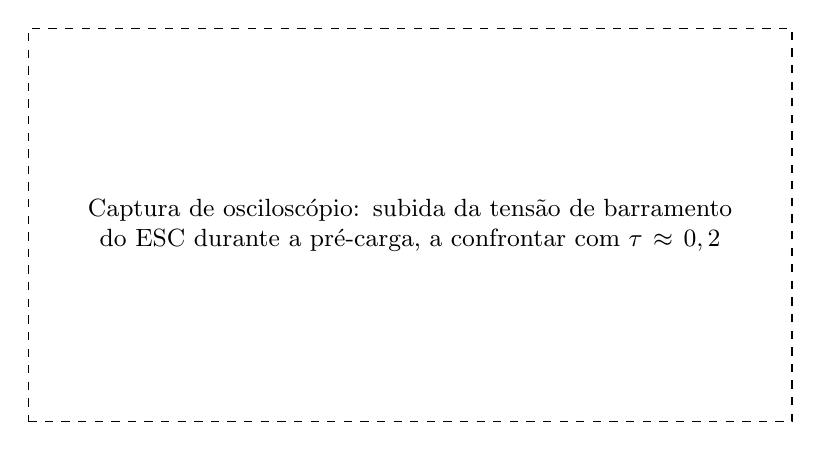
\begin{tikzpicture}
        \node[draw, dashed, align=center, minimum width=0.8\textwidth,
              minimum height=5cm, text width=0.7\textwidth, font=\small]
              {Captura de osciloscópio: subida da tensão de barramento do
               ESC durante a pré-carga, a confrontar com $\tau \approx
               \SI{0,2}{\second}$};
    \end{tikzpicture}

    Fonte: Autor (2026)
\end{figure}

\subsection{Caixa de Instrumentação}

A integração dos sistemas SAME e SIBA foi realizada em uma caixa de
instrumentação fabricada por impressão 3D em filamento PLA, projetada para
centralizar a alimentação, o processamento e as conexões de sinal em um único
módulo físico. A escolha da impressão 3D permitiu a prototipagem rápida de uma
geometria customizada às necessidades do projeto, com fixação interna dedicada
para cada subsistema. Por se tratar de ensaios de curta duração, a limitação
térmica do PLA não compromete a operação; ainda assim, previram-se aberturas
para dissipação do calor gerado pelos componentes de potência. O modelo
tridimensional da caixa está na \autoref{fig:cad_caixa}.

\begin{figure}[H]
    \centering
    \caption{Modelo em CAD da caixa de instrumentação (espaço reservado)}
    \label{fig:cad_caixa}
    \begin{tikzpicture}
        \node[draw, dashed, align=center, minimum width=0.8\textwidth,
              minimum height=6cm, text width=0.7\textwidth, font=\small]
              {Render do modelo CAD da caixa de instrumentação};
    \end{tikzpicture}

    Fonte: Autor (2026)
\end{figure}

\subsection{Organização Interna}

O \textit{layout} interno foi organizado de forma a separar fisicamente os
componentes de potência dos circuitos de medição, minimizando o acoplamento
eletromagnético entre eles. Tal separação é particularmente crítica neste
projeto, uma vez que os sinais de interesse são de baixa amplitude — como a
queda de tensão da ordem de milivolts sobre resistências de poucos
miliohms e a saída dos sensores de efeito Hall —, sendo, portanto,
suscetíveis a interferência. As placas SAME e SIBA foram fixadas nas
extremidades da caixa por meio de parafusos, enquanto a placa de
condicionamento de sinal do motor foi posicionada na região central,
equidistante das duas placas principais. O ESC foi fixado internamente por
abraçadeiras de náilon, garantindo imobilidade mecânica durante os ensaios
sem danificar o encapsulamento do componente.

O \textit{switch} Ethernet foi instalado internamente, com as portas RJ45
acessíveis pelo painel externo da caixa, permitindo a conexão com a rede de
aquisição sem necessidade de abertura do gabinete. A
\autoref{fig:montagem_interna} mostra essa organização.

\begin{figure}[H]
    \centering
    \caption{Organização interna da caixa de instrumentação (espaço reservado)}
    \label{fig:montagem_interna}
    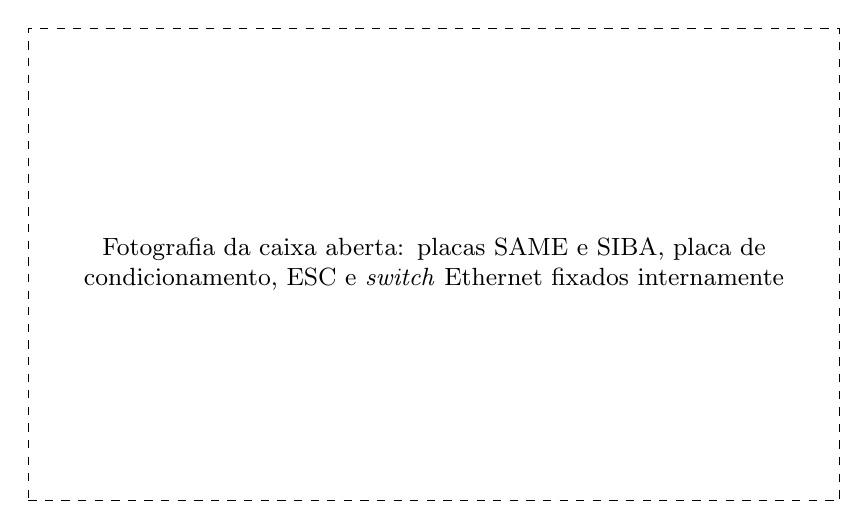
\begin{tikzpicture}
        \node[draw, dashed, align=center, minimum width=0.85\textwidth,
              minimum height=6cm, text width=0.75\textwidth, font=\small]
              {Fotografia da caixa aberta: placas SAME e SIBA, placa de
               condicionamento, ESC e \textit{switch} Ethernet fixados
               internamente};
    \end{tikzpicture}

    Fonte: Autor (2026)
\end{figure}

\subsection{Conexões Externas}

O painel externo da caixa concentra todas as interfaces com o ambiente de
ensaio. O conector XT90 de entrada recebe a bateria LiPo, enquanto um segundo
conector XT90 de saída alimenta o ESC. Os fios de fase do motor passam pelo
interior da caixa através de conectores \textit{bullet} de \SI{6}{\milli\meter},
permitindo a interposição dos núcleos de ferrite para a medição de corrente sem
interrupção do cabo de potência. Uma entrada dedicada no painel permite a
conexão dos fios da célula de carga utilizada para a medição de força de tração
na bancada aerodinâmica. A \autoref{fig:painel_externo} mostra o painel
montado.

\begin{figure}[H]
    \centering
    \caption{Painel externo com as conexões de potência, de sinal e de rede (espaço reservado)}
    \label{fig:painel_externo}
    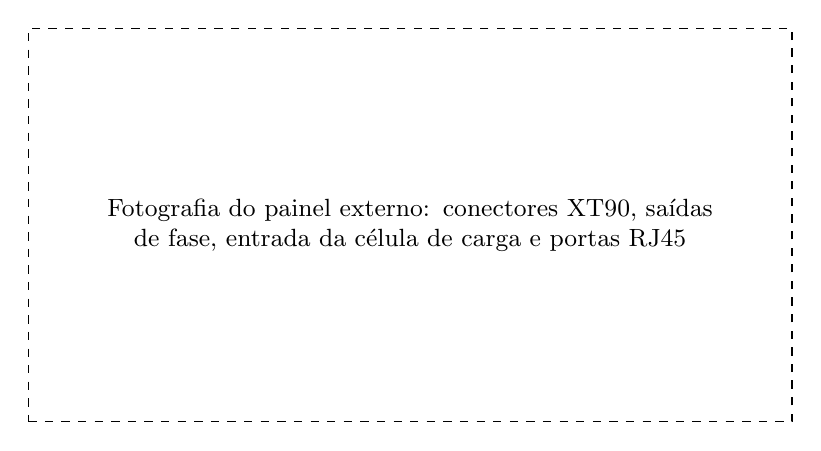
\begin{tikzpicture}
        \node[draw, dashed, align=center, minimum width=0.8\textwidth,
              minimum height=5cm, text width=0.7\textwidth, font=\small]
              {Fotografia do painel externo: conectores XT90, saídas de
               fase, entrada da célula de carga e portas RJ45};
    \end{tikzpicture}

    Fonte: Autor (2026)
\end{figure}
